
\section{Übertrangungsmedien}
\subsection{Ausbreitungsgeschwindigkeit}
{Lichtgeschwindigkeit im Vakuum:
    $$ c_0 = 299'792'458 m/s $$
}

{Ausbreitungsgeschwindigkeit in Medien: \\
    $$ c_{Medium} = 200'000 km/s = \frac{2}{3} c_0 $$}

\begin{tikzpicture}
    \node [examplebox] (box){
        \begin{minipage}{0.3\textwidth}
            {Licht im Glas, Brechnungsindex $n=1.5$}
            $$ c_{Glas} = \frac{c_0}{n} = 200'000 km/s  $$
        \end{minipage}
    };
    \node[exampletitle, right=8pt] at (box.north west) {Beispiel:};
\end{tikzpicture}
\subsection{Signaldämpfung}{
    {Signaldämpfung bezeichnet die Leistungsabnahme eines Signals.}
    \begin{itemize}[noitemsep]
        \item Je grösser die Bandbreite (Hz), desto höhere Datenraten (bit/s) übertragen
        \item Je kleiner die Dämpfung ist, desto grössere Distanzen können erreicht werden
        \item Senkt man die Bitrate (bei gleicher Dämpfung), können grössere Distanzen erreicht werden
    \end{itemize}}
$$ dB = 10 \cdot log(\frac{P_1}{P_2})$$
$$ dB = 10 \cdot log(\frac{U_1}{U_2})^2$$

\subsection{Signal-Rausch-Verhältnis (SNR)}{
    {Das SNR ist ein Mass für die Qualität eines Signals. Es gibt an, wie stark das Signal im Vergleich zum Rauschen ist. }
    $$ SNR = 10 \cdot log(\frac{P_{Signal}}{P_{Noise}}) $$
    In dB  angegeben.
}

\subsection{Signale und Störungen}{

    {\includegraphics[scale=.225]{img/Signale und Störungen.png}}

    Mögliche Ursachen der Störungen:
    \begin{itemize}[noitemsep]
        \item Übersprechen zwischen den Leitungen
        \item Rauschen des Empfängers
        \item Einstreuungen durch andere Geräte / Anlagen (Motoren etc.)
    \end{itemize}

}

\subsection{Kabeltypen}{
    \begin{itemize}[noitemsep]
        \item Koaxialkabel $\to$ Geeignet für hochfrequente Signale
        \item Twinaxial-Kabel $\to$ Hoher Schutz
        \item Twisted Pair (TP) $\to$ Häufig im Einsatz (Shielded / Unshielded)
        \item Glasfaser $\to$ Hohe Bandbreite, Geringe Dämpfung, Resistent
    \end{itemize}
}
\subsection{Schirmeigenschaften}
{ \begin{itemize}[noitemsep]
        \item Drahtgeflecht $\to$niederfrequente Einstreuungen
        \item Metallisch beschichtete Folien $\to$ hochfrequente Störungen
    \end{itemize}}
{   {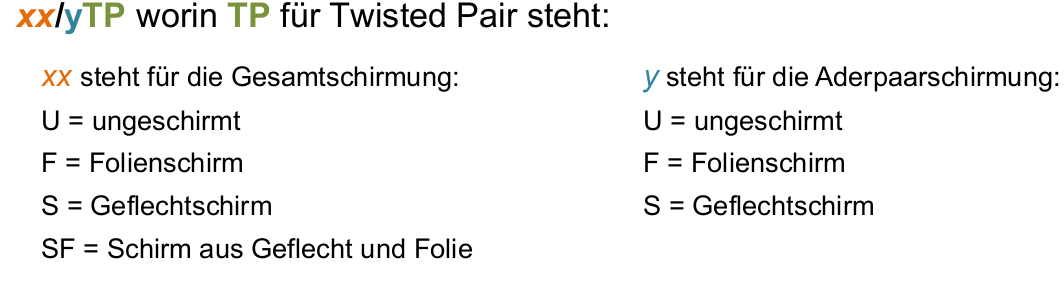
\includegraphics[scale=.225]{img/twisted.png}}}

\subsection{TP Kabel und Störungen}{
    \begin{itemize}[noitemsep]
        \item TP Kabel sind anfälliger auf Störungen als Koaxialkabel oder Glasfasern
        \item Störungen werden kapazitiv oder induktiv eingekoppelt z.B. von parallel geführten Leitungen oder Motoren etc.
        \item Bei Störungen von benachbarten Leitungen spricht man von Übersprechen oder
              Nebensprechen (crosstalk)
    \end{itemize}}
\begin{tikzpicture}
    \node [examplebox] (box){
        \begin{minipage}{0.3\textwidth}
            \begin{itemize}[noitemsep]
                \item Kappazitive Störung $\to$ Abschirmung
                \item Induktive Störung $\to$ twisted
            \end{itemize}
        \end{minipage}
    };
    \node[exampletitle, right=8pt] at (box.north west) {Fausregel:};
\end{tikzpicture}
\WhiteSpace

\subsection{Lichtwellenleiter}{
    { \begin{itemize}[noitemsep]
                \item Zentrum aus Kernglas mit hoher optischer Dichte (Brechungsindex 1.5)
                \item Vom Mantelglas umschlossen, geringere optische Dichte (Brechungsindex 1.48)
                \item Lichtstrahlen breiten sich im Kernglas aus und werden am Mantelglas totalreflektiert
                \item Die Eigenwellen (Ausbreitungswege der Lichtstrahlen) werden als Moden bezeichnet.
            \end{itemize}}
}